\documentclass[11pt]{article}

\usepackage{fancyhdr}
\usepackage{tipa}
\usepackage{fontspec}
\usepackage{amsfonts}
\usepackage{enumitem}
\usepackage[margin=1in]{geometry}
\usepackage{graphicx}
\usepackage{float}
\usepackage{amsmath}
\usepackage{braket}
\usepackage{amssymb}
\usepackage{booktabs}
\usepackage{hyperref}
\usepackage{mathtools}
\usepackage{float}
\usepackage{algpseudocodex}
\usepackage{titlesec}
\usepackage{bbm}

\newcommand{\cnum}{ECE M146}
\newcommand{\ced}{Spring 2023}
\newcommand{\ctitle}[4]{\title{\vspace{-0.5in}\cnum, \ced\\Problem Set #1: #2}\author{\vspace{-0.35in}\\Name: #3, UID: #4}}
\newcommand{\solution}[1]{{{\color{blue}{\bf Solution:} {#1}}}}

\renewcommand*{\theenumi}{\alph{enumi}}
\renewcommand*\labelenumi{(\theenumi)}
\renewcommand*{\theenumii}{\roman{enumii}}
\renewcommand*\labelenumii{\theenumii.}

\newcommand{\R}{\mathbb{R}}
\newcommand{\norm}[1]{\left\lVert#1\right\rVert}

\DeclareMathOperator{\Cov}{Cov}
\DeclareMathOperator{\Var}{Var}
\DeclareMathOperator{\E}{E}
\DeclareMathOperator{\Tr}{Tr}
\DeclareMathOperator{\sign}{sign}


\begin{document}
\ctitle{2}{SVM}{Kevin Sheng}{406 196 414}
\date{}
\maketitle

\section{Problem 1}

\subsection{Problem 1a}

\solution{
      The closest the two classes get to each other is with $x_1=-1$ and $x_5=-2$.

      The slope between them is $\frac{1-4}{-1-2}=-3$,
      and their midpoint is $\left(-\frac{3}{2}, \frac{5}{2}\right)$.

      This makes the point-slope equation of the line
      \[\frac{y_2-\frac{5}{2}}{y_1+\frac{3}{2}}=-3\]
      and the normal equation of the line
      \[\boxed{-\frac{y_1}{3}+y_2-3=0}\]
      The margin of the hyperplane is the distance from
      the two points I talked about above to the midpoint, so it's
      gotta be $\sqrt{\left(\frac{1}{2}\right)^2+\frac{3}{2}^2}=\boxed{\frac{\sqrt{10}}{2}}$.
}

\pagebreak

\subsection{Problem 1b}

\solution{
      \begin{figure}[h]
            \centering
            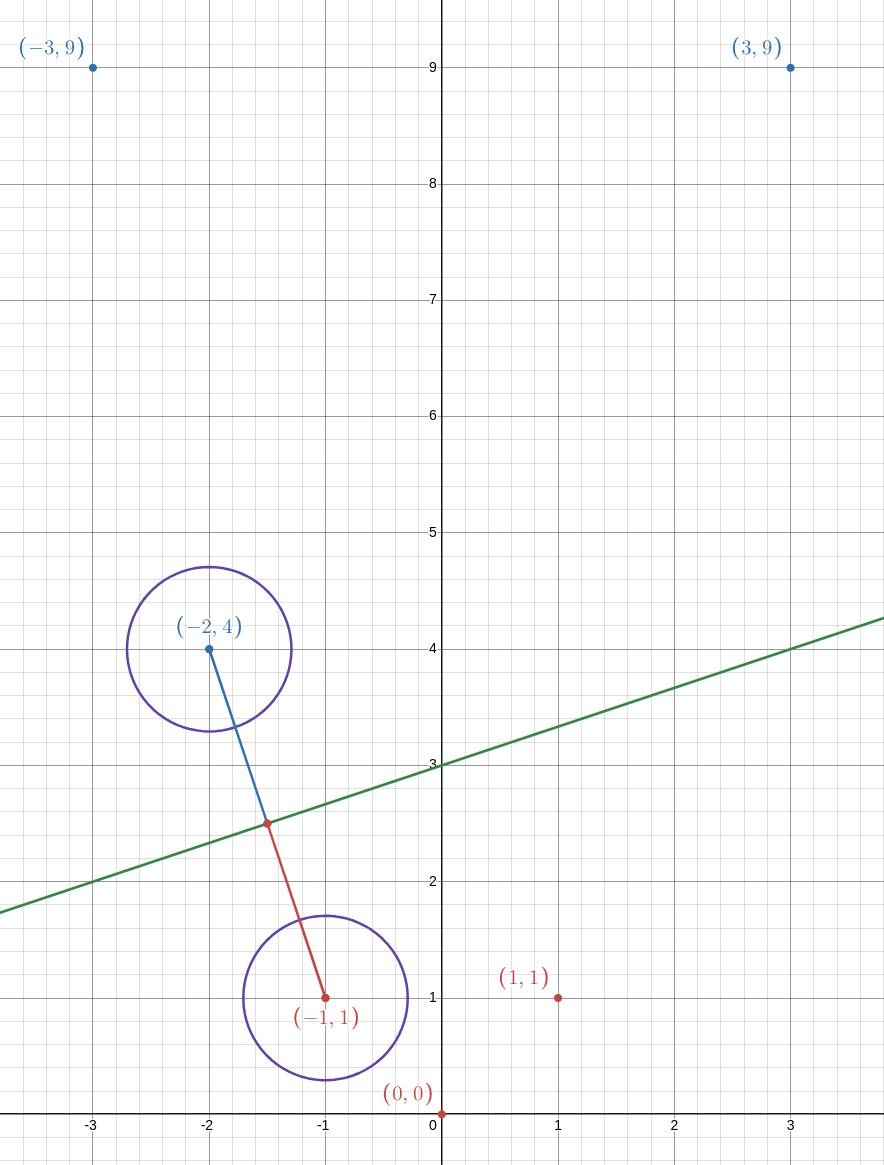
\includegraphics[width=12cm]{img/hw3/svm}
            \caption{
                  All the points with the separating hyperplane.
                  The red points are the negative examples and the blue points are the positive examples.
            }
      \end{figure}
}

\pagebreak

\subsection{Problem 1c}

\solution{
      \begin{figure}[h]
            \centering
            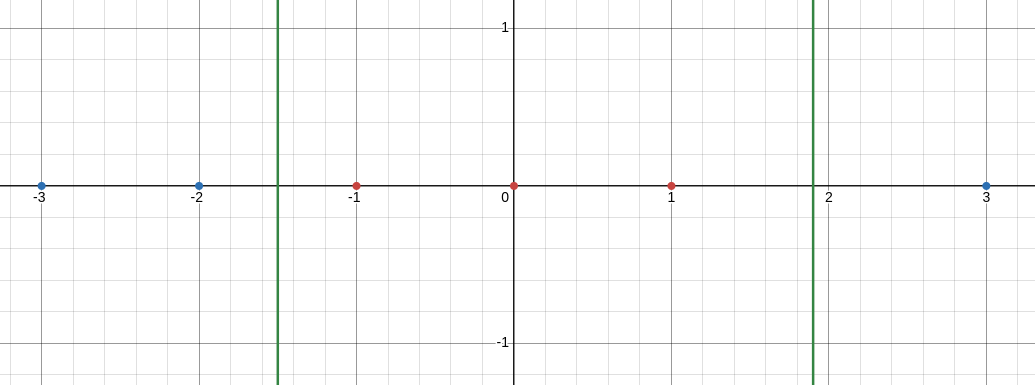
\includegraphics[width=12cm]{img/hw3/decision}
            \caption{The same points but mapped back to $\R$.}
      \end{figure}
}

\subsection{Problem 1d}

\solution{
      As we can see, there's only two points in the dataset that actually matter.
      Thus, we only have to consider their $\alpha$ terms in the dual:
      \begin{gather*}
            \max_{\alpha} \alpha_1+\alpha_5+\frac{1}{2}\alpha_1\alpha_5\phi(x_1)^T\phi(x_5)\text{ s.t.} \\
            0 \le \alpha \le C\ \forall i=1, \cdots, n \\
            \alpha_1 - \alpha_5 = 0
      \end{gather*}

      The data is linearly separable, so it doesn't matter what $C$ is-
      if we arbitrarily set it as $C$, then $\alpha_1=\alpha_5=1$.

      % ok like this formula literally doesn't work and i have NO CLUE WHY
      Plugging these $\alpha$s into the formulas derived in class we see that
      \[w=\sum_{n=1}^{5} y_n\alpha_n\phi(x_n)=-\begin{bmatrix}-1 \\ 1\end{bmatrix}
            +\begin{bmatrix}-2 \\ 4\end{bmatrix}
            =\begin{bmatrix}-1 \\ 3\end{bmatrix}\]
      and that $b=\boxed{-9}$.
}

\subsection{Problem 1e}

\solution{
      Adding a negative example at $x=0.5$ won't change anything
      because the SVM still correctly classifies it and it's also far
      from the boundary.
}

\pagebreak

\section{Problem 2}

\subsection{Problem 2a}

\solution{
      First we turn everything into its conventional form:
      \begin{gather*}
            1 - \xi_i - y_i\left(w^Tx_i+b\right) \le 0 \\
            -\xi_i \le 0
      \end{gather*}

      Then, applying the formula from lecture gives us
      \begin{align*}
                & \mathcal{L}(w, b, \xi, \alpha, \lambda)       \\
            ={} & \frac{1}{2}\norm{w}^2+\sum_{i=1}^{n} C_i\xi_i
            +\sum_{i=1}^{n} \alpha_i\left(1 - \xi_i - y_i\left(w^Tx_i+b\right)\right)
            +\sum_{i=1}^{n} -\lambda_i\xi_i                     \\
            ={} & \frac{1}{2}\norm{w}^2+\sum_{i=1}^{n} C_i\xi_i
            -\sum_{i=1}^{n} \alpha_i\left(y_i\left(w^Tx_i+b\right)-1+\xi_i\right)
            -\sum_{i=1}^{n} \lambda_i\xi_i \quad\square
      \end{align*}

      As always we have the constraints where
      \begin{align*}
            \alpha_i \ge 0 &  & \lambda_i \ge 0
      \end{align*}
}

\subsection{Problem 2b}

\solution{
      \begin{enumerate}[label=\roman*.]
            \item The gradent w.r.t $w$ is
                  \begin{align*}
                        \nabla_w \mathcal{L}
                         & = \nabla_w \frac{1}{2}\norm{w}^2
                        - \sum_{i=1}^{n} \nabla_w \alpha_i y_i \left(w^T x_i\right) \\
                         & = w - \sum_{i=1}^{n} \alpha_i y_i x_i
                  \end{align*}
                  Setting it to $0$ gives us
                  \[w=\sum_{i=1}^{n} \alpha_i y_i x_i\]

            \item The grad wrt $b$ is just
                  \[\nabla_w \mathcal{L}
                        = -\sum_{i=1}^{n} \nabla_b \alpha_i y_i b \\
                        = -\sum_{i=1}^{n} \alpha_i y_i\]
                  so this summation has to be $0$ as well.

            \item From inspection it's clear that
                  \begin{align*}
                        \nabla_{\xi_i} \mathcal{L} = C_i - \alpha_i - \lambda_i
                        \implies{} C_i = \alpha_i + \lambda_i
                  \end{align*}
      \end{enumerate}
}

\pagebreak

\subsection{Problem 2c}

\solution{
      Putting the equations back into the objective function gives us
      \begin{align*}
            \mathcal{L}
             & = \frac{1}{2}\norm{w}^2+\sum_{i=1}^{n} C_i\xi_i
            -\sum_{i=1}^{n} \alpha_i\left(y_i\left(w^Tx_i+b\right)-1+\xi_i\right)
            -\sum_{i=1}^{n} \lambda_i\xi_i                                                              \\
             & = \frac{1}{2}\norm{w}^2 + \sum_{i=1}^{n} \xi_i(C_i-\alpha_i-\lambda_i)
            - \sum_{i=1}^{n} \left(\alpha_i y_i \left(w^T x_i + b\right) - \alpha_i\right)              \\
             & = \frac{w^T w}{2}
            - \sum_{i=1}^{n} \left(\alpha_i y_i \left(w^T x_i + b\right) - \alpha_i\right)              \\
             & = \frac{w^T w}{2}
            - w^T \sum_{i=1}^{n} \alpha_i y_i x_i
            - b \sum_{i=1}^{n} \alpha_i y_i
            + \sum_{i=1}^{n} \alpha_i                                                                   \\
             & = \frac{w^T w}{2} - w^T w + \sum_{i=1}^{n} \alpha_i                                      \\
             & = -\frac{w^T w}{2} + \sum_{i=1}^{n} \alpha_i                                             \\
             & = -\frac{1}{2} \sum_{i=1}^{n} \sum_{j=1}^{n} \alpha_i\alpha_jy_iy_j\left(x_i^Tx_j\right)
            + \sum_{i=1}^{n} \alpha_i\quad\square
      \end{align*}
}

\subsection{Problem 2d}

\solution{
      The actual problem is as follows:
      \begin{gather*}
            \min_{\alpha} \sum_{i=1}^{n} \alpha_i
            -\frac{1}{2} \sum_{i=1}^{n} \sum_{j=1}^{n} \alpha_i\alpha_jy_iy_j\left(x_i^Tx_j\right)
            \text{ s.t.} \\
            0 \le \alpha_i \le C_i\ \forall i=1, \cdots, n \\
            \sum_{i=1}^{n} \alpha_i y_i = 0
      \end{gather*}
}

\subsection{Problem 2e}

\solution{
      Since everything is written in terms of dot products on $x_i$,
      this problem is kernelizable.
      In fact, the only difference between this dual and the original SVM dual
      is that instead of a constant $C$ in the contraints we have a $C_i$ instead.
}

\pagebreak

\section{Problem 3}

\subsection{Problem 3a}

\solution{
      One of the best classifiers is $h_1(x)=\sign(x_2-3.5)$,
      which only gets the positive instance at $(5, 1)$ wrong.
      Its error is only $0.2$, so its contribution is $\beta_1=\frac{1}{2}\ln 4$.
}

\subsection{Problem 3b}

\solution{
      An optimal classifier after the weight updates is $h_2(x)=\sign(x_1-4.5)$.
      This one gets the points at $(1, 5)$ and $(2, 4)$ wrong, so its error is $0.25$
      and its contribution is $\beta_2=\frac{1}{2}\ln 3$.
}

\subsection{Problem 3c}

\solution{
      Our final classifier is
      \[h(x)=\sign\left[\frac{\ln 4}{2}\sign(x_2-3.5)+\frac{\ln 3}{2}\sign(x_1-4.5)\right]\]
}

\subsection{Completed Table}

The final table after both these iterations is below:
\begin{table}[H]
      \centering
      \begin{tabular}{|c|c|c|c|c|c|c|c|c|c|}
            \hline
            \textbf{Sample} & \textbf{Label} & $x_1$ & $x_2$ & $\hat{y}_1^{(1)}$ & $\epsilon^{(1)}$ & $w^{(1)}$ & $\hat{y}_2^{(1)}$ & $\epsilon^{(2)}$ & $\hat{y}$ \\
            \hline
            1               & 1              & 1     & 5     & 1                 & 0                & 0.125     & -1                & 0.125            & 1         \\
            \hline
            2               & 1              & 2     & 4     & 1                 & 0                & 0.125     & -1                & 0.125            & 1         \\
            \hline
            3               & -1             & 3     & 3     & -1                & 0                & 0.125     & -1                & 0                & -1        \\
            \hline
            4               & -1             & 4     & 2     & -1                & 0                & 0.125     & -1                & 0                & -1        \\
            \hline
            5               & 1              & 5     & 1     & -1                & 0.2              & 0.5       & 1                 & 0                & -1        \\
            \hline
      \end{tabular}
\end{table}

\end{document}
